\documentclass[handout]{beamer}

\usepackage{float}
\usepackage{graphicx}
\usepackage{url}

\usepackage{../cppenv}

\usepackage{../recdefs}

\usetheme{Berkeley}

\title{CS100 Recitation 2}
\author{GKxx}
\date{Februrary 28, 2022}

\begin{document}

\begin{frame}
    \maketitle
\end{frame}

\AtBeginSection[]{
    \begin{frame}{Contents}
        \tableofcontents[currentsection]
    \end{frame}
}

\section{Operators}

\begin{frame}[fragile]{\ttt{++} and \ttt{--}}
    Increment and decrement operators
    \begin{itemize}
        \item Both \ttt{i++} and \ttt{++i} increases the value of \ttt{i} by \ttt{1}.
        \pause
        \item What are the values of \ttt{i}, \ttt{j} and \ttt{k} after the following code is executed?
        \begin{cpp}
int i = 42;
int j = ++i;
int k = i++;
        \end{cpp}
        \pause
        \blue{\ttt{i == 44, j == 43, k == 43}.}
    \end{itemize}
\end{frame}

\begin{frame}[fragile]{\ttt{++} and \ttt{--}}
    \begin{itemize}
        \item What are the values of \ttt{j} and \ttt{k}?
        \begin{cpp}
int i = 42;
int j = ++i, k = i++;
        \end{cpp}
        \pause
        \blue{\ttt{j == 43, k == 43}.}
        \pause
        \item What's the output of the following code?
        \begin{cpp}
int i = 42;
printf("%d, %d", ++i, i++);
        \end{cpp}
        \pause
        \red{Undefined behavior!}
    \end{itemize}
\end{frame}

\begin{frame}[fragile]{\ttt{++} and \ttt{--}}
    The \blue{prefix} increment operator:
    \begin{enumerate}
        \item Increases the value of the variable.
        \item Returns the \blue{variable}.
    \end{enumerate}
    \pause
    The \blue{postfix} increment operator:
    \begin{enumerate}
        \item Saves the original value of the variable.
        \item Increases the value of the variable.
        \item Returns the original \blue{value} that has been saved.
    \end{enumerate}
    \pause
    \begin{itemize}
        \item More about the difference between them will be discussed in the C++ part.
    \end{itemize}
\end{frame}

\begin{frame}{Relational Operators}
    Relational Operators: \ttt{<}, \ttt{<=}, \ttt{>}, \ttt{>=}, \redtt{==}, \ttt{!=}.
    \begin{itemize}
        \item What is the return-type of these operators?\\
        \pause
        \blue{Unfortunately it is \ttt{int} instead of \ttt{bool}, due to the problematic definitions of \ttt{true} and \ttt{false} before C23.}\\
        \blue{In C++, it is undoubtedly \ttt{bool}.}
        \pause
        \item What's the result of the expression \ttt{a < b < c}?\\
        \pause
        \blue{It behaves as expected in Python, but not in C.}
    \end{itemize}
\end{frame}

\begin{frame}{Arithmetic Operators}
    Arithmetic Operators: \ttt{+} (unary/binary), \ttt{-} (unary/binary), \ttt{*}, \ttt{/}, \ttt{\%}, as well as bitwise operators \ttt{\&}, \ttt{\^{}}, \ttt{|}, \ttt{\~}, \ttt{<<}, \ttt{>>}.
    \begin{itemize}
        \item If at least one of the operands is \blue{floating-point}, the other integer operand, if any, will be converted to the same floating-point type. (More about type conversion will be discussed later.)
        \pause
        \item Division for integers:
        \begin{itemize}
            \item Rounded in \blue{implementation-defined} direction. \red{(Until C99)}
            \item Truncated towards zero. \red{(Since C99)}
            \item e.g. \ttt{3 / -2 == -1} (since C99)
        \end{itemize}
        \item Remainder: \ttt{(a / b) * b + a \% b == a} is always true.
        \pause
        \item Bitwise operators will be discussed in the next recitation.
    \end{itemize}
\end{frame}

\begin{frame}{Compound Assignment Operators}
    Compound assignment operators: \ttt{+=}, \ttt{-=}, \ttt{*=}, \ttt{/=}, \ttt{\%=}, \blue{\ttt{<<=}, \ttt{>>=}, \ttt{\&=}, \ttt{|=}, \ttt{\^{}=}}.
    \begin{itemize}
        \item `\ttt{a = a op b}' is the same as `\ttt{a op= b}'.
        \item Practice to use them more, as they are clear and increases readability.
    \end{itemize}
\end{frame}

\begin{frame}{Conditional Operator}
    Conditional operator: \ttt{cond ? exprT : exprF}.
    \begin{itemize}
        \item The evaluation order is determined!
        \pause
        \begin{itemize}
            \item \ttt{cond} will be evaluated first. If \ttt{cond} evaluates \bluett{true}, \ttt{exprT} will be evaluated, otherwise \ttt{exprF} will be evaluated.
            \item Only one of \ttt{exprT} and \ttt{exprF} will be evaluated.
        \end{itemize}
        \pause
        \item It is suggested to use it for simple occasions like `\ttt{a < b ? a : b}'.
        \item Nested conditional expressions reduces the readability sharply!
        \begin{itemize}
            \item \ttt{a < b ? (a < c ? a : c) : (b < c ? b : c)}
        \end{itemize}
    \end{itemize}
\end{frame}

\section{IO}

\begin{frame}{\ttt{scanf} and \ttt{printf}}
    For the authoritative reference, view it on \url{https://en.cppreference.com/w/c/io/fscanf} and \url{https://en.cppreference.com/w/c/io/fprintf}.\\
    \pause
    Some common issues:
    \begin{itemize}
        \item You should always make sure that the format string and the variables \textbf{match} each other, especially in \bluett{scanf}!
        \item More details about mismatch will be discussed after you have learned pointers and conversions.
        \pause
        \item Any \blue{whitespace character} consumes all available \blue{consecutive} whitespace characters. So the statement \ttt{scanf("\%d\textbackslash n", \&a);} keeps waiting for the next non-whitespace character.
    \end{itemize}
\end{frame}

\begin{frame}[fragile]{\ttt{scanf} and \ttt{printf}}
    \begin{itemize}
        \item Preceeding whitespaces will be ignored when matching conversion specifiers \blue{(beginning with `\%')}, but \textbf{will not be ignored} when matching other characters!
        \begin{itemize}
            \item \ttt{scanf("(\%d,\%d)", \&a, \&b);}
            \item If `\ttt{(3, 2)}' is inputted, the space before `\ttt{2}' will be ignored.
            \pause
            \item What about this?
            \begin{cpp}
for (int i = 0; i < n; ++i)
    scanf("(%d,%d)", &a, &b);
            \end{cpp}
            \pause
            \blue{If the data is inputted line-by-line, the first input stops at the first newline character.}\\
            \blue{Then that newline character is read in the second iteration, which does not match `\ttt{(}'. Thus a failure occurs.}\\
            \pause
            To solve this, write \redtt{scanf(" (\%d,\%d)", \&a, \&b);}.
        \end{itemize}
    \end{itemize}
\end{frame}

\begin{frame}{\ttt{scanf} and \ttt{printf}}
    \begin{itemize}
        \item \ttt{scanf("\%c", \&a);} does not ignore preceeding whitespaces! (You may have a try on your own.)
        \pause
        \item \ttt{scanf} returns an \bluett{int} value, denoting the number of receiving arguments successfully assigned, or \bluett{EOF} (-1) if input failure occurs before the first receiving argument was assigned.
        \item You can use the return-value to detect failure of \ttt{scanf}.
        \begin{itemize}
            \item \ttt{int r = scanf("(\%d,\%d)", \&a, \&b);}
            \item If two integers are read and assigned successfully, \ttt{r} will be assigned \ttt{2}.
        \end{itemize}
    \end{itemize}
\end{frame}

\section{Control flow}

\begin{frame}[fragile]{\ttt{if}-\ttt{else}}
    \begin{itemize}
        \item Which \ttt{if} does the \ttt{else} match?
        \begin{cpp}
if (a == b)
    if (c < d)
        do_something();
else
    do_another_thing();
        \end{cpp}
        \pause
        \item Dangling \ttt{else}!
    \end{itemize}
\end{frame}

\begin{frame}[fragile]{\ttt{if}-\ttt{else}}
    \begin{itemize}
        \item Use \bluett{else} properly to avoid repeated calculation, and also make your code more robust.
        \begin{cpp}
if (b == 0)
    printf("Error: Division by zero!\n");
if (b != 0) // Better to use `else' here!
    printf("The answer is %lf\n", a / b);
        \end{cpp}
    \end{itemize}
\end{frame}

\begin{frame}[fragile]{\ttt{if}-\ttt{else}}
    \begin{alertblock}{Interesting fact}
        The `\ttt{)}' is used to separete the condition and the statement. The only reason for writing `\ttt{(}' is to match the `\ttt{)}'.
    \end{alertblock}
    \ttt{if}-\ttt{else} in Python:
    \begin{cpp}
if condition:
    statement
    \end{cpp}
    In Pascal:
    \begin{cpp}
if condition then
    statement
    \end{cpp}
\end{frame}

\begin{frame}[fragile]{\ttt{for} loop}
    \begin{cpp}
for (init-expression; condition; expression)
    statement
    \end{cpp}
    \begin{itemize}
        \item Since C99, variable declaration is allowed in the `init-expression' part.
        \begin{cpp}
for (int i = 0; i < n; ++i)
    do_something();
        \end{cpp}
        \pause
        \item The variable \ttt{i} is declared in the \bluett{for} loop, and destroyed immediately the loop ends.
        \begin{cpp}
for (int i = 0; i < n; ++i)
    do_something();
printf("%d\n", i); // Error: i was not declared in this scope.
        \end{cpp}
    \end{itemize}
\end{frame}

\begin{frame}{The self-teach algorithm}
    \begin{figure}[htbp]
        \centering
        \begin{minipage}{0.3\textwidth}
            \centering
            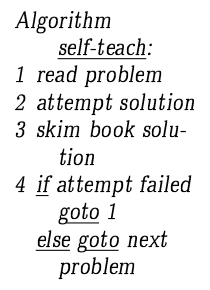
\includegraphics[width=0.9\textwidth]{img/self-teach.png}
        \end{minipage}
        \begin{minipage}{0.3\textwidth}
            \centering
            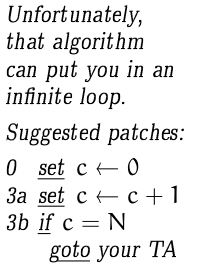
\includegraphics[width=0.9\textwidth]{img/self-teach2.png}
        \end{minipage}
        \begin{minipage}{0.3\textwidth}
            \centering
            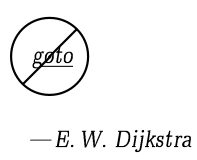
\includegraphics[width=0.9\textwidth]{img/nogoto.png}
        \end{minipage}\\
        (In \textit{Concrete Mathematics}, Chapter 5 Section 2.)
    \end{figure}
\end{frame}

\section{Variables}

\begin{frame}{Variable naming}
    \begin{itemize}
        \item \ttt{int num\_of\_student;}
        \item \ttt{int numOfStudent;}
        \item \ttt{\#define SIZE 128}
        \pause
        \item The names of normal variables or functions are recommended to begin in lower case.
        \item Macros are often named in upper case.
        \pause
        \item \blue{Similar rules apply to the names of folders and files!}
    \end{itemize}
\end{frame}

\begin{frame}{Variable declaration}
    \begin{itemize}
        \item In C89, variables declarations are only allowed at the beginning of blocks.
        \item This requirement is removed since C99.
        \begin{figure}[h]
            \centering
            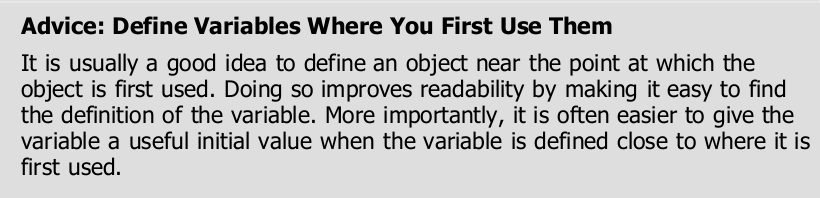
\includegraphics[width=0.9\textwidth]{img/advice-variables.png}
        \end{figure}
    \end{itemize}
\end{frame}

\begin{frame}{Variable initialization}
    \red{You must remember the following firmly!}
    \begin{itemize}
        \item Local non-static variables, if not \blue{explicitly initialized}, will be \blue{default initialized}, that is, initialized with an \red{underined} value.
        \item Global variables or local static variables, if not \blue{explicitly initialized}, will be \blue{value initialized}, that is, initialized with zero. (character types and integer types: \ttt{0}; floating-point types: \ttt{0.0}; pointers: \ttt{NULL}).
        \pause
        \item Arrays are initialized element-by-element according to the same rule above.
        \item Additional rule for arrays: For local non-static arrays, if an explicit initializer is provided but \blue{it does not cover all the elements of the array}, those elements not covered will be \blue{value initialized}!
    \end{itemize}
\end{frame}

\end{document}